\documentclass[12pt,a4paper]{article}
\usepackage{amsmath,amssymb,amsthm}
\usepackage{graphicx}
\usepackage{booktabs}
\usepackage{hyperref}
\usepackage{natbib}
\usepackage[margin=2.5cm]{geometry}

\title{A CrossDomain Gap Analysis Reveals an Unexplored Mathematical
Framework for Regional Climate Prediction: Nash Equilibrium,
Stochastic Field Theory, and Formal Verification}

\author{Jes\'{u}s Isaac Castillo-S\'{a}nchez\\
\small Universidad Aut\'{o}noma Chapingo, Texcoco, M\'{e}xico\\
\small jcastillos@chapingo.mx\\
\small ORCID: 0009-0009-6913-0456}

\date{June 2026}

\graphicspath{{./}}
\begin{document}
\sloppy
\maketitle

\begin{abstract}
We present a systematic cross-domain gap analysis of 187 peer-reviewed
articles spanning six knowledge domains: climate prediction, game theory
(Nash equilibrium), stochastic differential equations, formal verification,
physics-informed machine learning~\citep{Raissi2019}, and regional climatology of Mexico.
Using the SCIFLOW CrossDomain-Matrix methodology and 24 structured Scopus
queries organized in four specificity levels, we identify 11 confirmed
literature gaps, including a Super-Gap at the triple intersection of
Nash equilibrium theory, stochastic field equations (Fokker-Planck/Langevin),
and formal mathematical verification applied to regional climate prediction.
While Nash equilibrium appears extensively in climate diplomacy (20 papers;~\citealt{Forgo2005})
and carbon markets (11 papers;~\citealt{Haurie2004}), it has never been applied as a physical
principle governing competing atmospheric mass dynamics. Similarly,
stochastic primitive equations exist mathematically \citep{Debussche2012,
Majda2006} but without Nash solutions or formal verification.
We propose a theoretical framework --- the Nash-EDE Climate Model (NECM) ---
that fills this gap, derive its core falsifiable prediction
($\gamma_{PG}/\sqrt{\beta_P\beta_G} \in [1.2, 2.5]$ distinguishes
stable bimodal precipitation regimes), and outline a research agenda
of seven articles derivable from this foundation.
\end{abstract}


\section{Methodology}

\subsection{Corpus Construction}

We constructed a multi-domain corpus by querying the Scopus database
(accessed June 23, 2026) across six knowledge domains: (1) regional
climate prediction, (2) Nash equilibrium and game theory, (3) stochastic
differential equations applied to atmospheric dynamics, (4) formal
mathematical verification, (5) physics-informed machine learning, and
(6) regional climatology of Mexico. Domain selection was guided by the
hypothesis that the intersection of Nash equilibrium theory, stochastic
field equations, and formal verification represents an unexplored
mathematical space for climate modeling.

Article retrieval was performed using the SCIFLOW CrossDomain-Matrix
methodology, an automated pipeline that structures literature queries in
four specificity levels and systematically identifies empty intersections
between domains. A total of 24 Scopus queries (S01--S24) were executed,
retrieving 190 records after deduplication by DOI, yielding 187 unique
articles for analysis.

\subsection{Four-Level Query Matrix}

Queries were organized in four levels of increasing specificity
(Table~\ref{tab:queries}):

\textbf{Level 1 — Base fields} (S01--S06): Single-domain queries
establishing that active literature exists in each individual domain.
This level confirms editorial receptivity and rules out the trivial
case of no prior work.

\textbf{Level 2 — Pairwise intersections} (S07--S14): Queries crossing
exactly two domains. A zero result at this level indicates a binary gap
— two fields that have never been connected in the literature.

\textbf{Level 3 — Triple intersections} (S15--S20): Queries crossing
three domains simultaneously. Zero results confirm that no prior work
has attempted the three-way synthesis.

\textbf{Level 4 — The Super-Gap} (S21--S24): Queries requiring the
simultaneous presence of Nash equilibrium, stochastic dynamics, climate
prediction, and formal verification. Zero results at this level, combined
with non-zero results at Level 1, constitute what we term a
\textit{confirmed Super-Gap}: a literature void bounded on all sides
by active fields.

\subsection{Thematic Classification}

Retrieved articles were classified into eight thematic categories using
keyword and abstract matching: Nash-diplomatic, Nash-economic,
Nash-physical-atmospheric, stochastic-climate, PINN-ML-climate,
Fokker-Planck-climate, formal-verification-climate, and Mexico-regional.
Classification was performed automatically via the SCIFLOW
ScientificKnowledgeExtractor module, with manual verification of
boundary cases.

\subsection{False Positive Detection Protocol}

Query S23 returned three results apparently linking Nash and Lean with
climate or physics. Manual inspection confirmed all three to be false
positives: the term ``Nash'' referred to the Nash-Sutcliffe efficiency
index~\citep{Nash1950}, a standard hydrological performance metric, and
``lean'' appeared in the sense of ``lean season'' or ``lean year'' in
hydroclimatological contexts. No paper in the corpus applies Nash
equilibrium from game theory alongside formal theorem provers such as
LeanFour2021 to any physical or climate model. This false-positive detection
step is a required component of the CrossDomain-Matrix protocol.

% FIGURA 1 placeholder
\begin{table}[ht]
\centering
\caption{Four-level query matrix S01--S24 with Scopus result counts
(June 23, 2026). Zero results confirm literature gaps; non-zero results
at Level 1 confirm editorial receptivity.}
\label{tab:queries}
\small
\begin{tabular}{llr}
\hline
\textbf{ID} & \textbf{Domain intersection} & \textbf{Results} \\
\hline
\multicolumn{3}{l}{\textit{Level 1 — Base fields}} \\
S01 & Climate prediction + Mexico + regional          &  48 \\
S02 & Atmospheric dynamics + stochastic + ODE         &  12 \\
S03 & Nash equilibrium + game theory + climate        &  70 \\
S04 & LeanFour2021 / formal verification + physics           &   8 \\
S05 & Physics-informed neural network + climate       &  62 \\
S06 & Fokker-Planck + atmospheric + temperature       &   5 \\
\hline
\multicolumn{3}{l}{\textit{Level 2 — Pairwise intersections}} \\
S07 & Nash equilibrium + competing air masses         &   \textbf{0} \\
S08 & Game theory + climate system + stability        &   1 \\
S09 & Stochastic ODE + climate + first principles     &   1 \\
S10 & Langevin + atmospheric temperature fluctuation  &   \textbf{0} \\
S11 & Formal verification + climate model             &   \textbf{0} \\
S12 & Lean/Coq/Isabelle + physics + verified          &  15 \\
S13 & Phase transition + climate + coexistence        &   \textbf{0} \\
S14 & Order parameter + atmospheric regime            &   4 \\
\hline
\multicolumn{3}{l}{\textit{Level 3 — Triple intersections}} \\
S15 & Nash + climate + stochastic                     &  48 \\
S16 & Game theory + atmospheric + Fokker-Planck       &   \textbf{0} \\
S17 & Nash equilibrium + air mass + prediction        &   \textbf{0} \\
S18 & Climate + mathematical proof + verified         &   \textbf{0} \\
S19 & Order parameter + climate + Ginzburg-Landau     &   1 \\
S20 & Competing phases + atmosphere + equilibrium     &   \textbf{0} \\
\hline
\multicolumn{3}{l}{\textit{Level 4 — Super-Gap}} \\
S21 & Nash + stochastic + climate + prediction        &   \textbf{0} \\
S22 & Game theory + Fokker-Planck + atmosphere        &   \textbf{0} \\
S23 & Nash + Lean + climate/physics                   &   3$^*$ \\
S24 & Formal verification + stochastic + climate      &   \textbf{0} \\
\hline
\multicolumn{3}{l}{$^*$ False positives: Nash-Sutcliffe index,
not Nash equilibrium.} \\
\hline
\end{tabular}
\end{table}

% ═══════════════════════════════════════════════════════
\section{Results}

\subsection{Level 1: Active Literature in All Base Fields}

All six base-field queries returned non-zero results, confirming that
each individual domain has an active publication record and established
editorial outlets. Climate prediction applied to Mexico (S01~=~48)
and physics-informed neural networks for climate (S05~=~62) show
particularly strong activity. Nash equilibrium and game theory in climate
contexts (S03~=~70) is the most active base field, establishing that
the concept of strategic interaction is not foreign to climate science.
Formal verification in physics (S04~=~8) and Fokker-Planck applied to
atmospheric systems (S06~=~5) are smaller but present fields, confirming
that the mathematical tools we propose are known, if rarely applied to
climate.

\subsection{Level 2: Four Binary Gaps Confirmed}

Of eight pairwise queries, four returned zero results:

\textbf{S07~=~0}: Nash equilibrium has never been applied to competing
atmospheric air masses. The 70 papers retrieved by S03 use Nash
exclusively in diplomatic or economic contexts (see Section~3.4).

\textbf{S10~=~0}: The Langevin equation, the stochastic differential
equation governing Brownian-type fluctuations, has never been applied
to atmospheric temperature fluctuations in the literature. This is
particularly notable given that atmospheric boundary-layer turbulence
is a canonical example of stochastic forcing~\citep{Hasselmann1976}.

\textbf{S11~=~0}: No climate model has ever been subjected to formal
mathematical verification using theorem provers. This gap persists
despite the fact that formal verification has been applied to aerospace~\citep{ModelChecking2018}
software, numerical algorithms, and recently to combustion models
\citep{LeanFour2021}.

\textbf{S13~=~0}: Phase transition formalism — including order parameters,
bifurcation diagrams, and coexistence conditions — has never been applied
to climate regime transitions. This is striking because the transition
between dry-season and wet-season dominance in tropical and subtropical
regions is phenomenologically identical to a thermodynamic phase transition.

\subsection{Level 3: Four Triple Gaps Confirmed}

\textbf{S16~=~0}: Game theory combined with both atmospheric science and
Fokker-Planck dynamics yields zero results. This triple intersection
is the mathematical core of the proposed Nash-EDE Climate Model (NECM).

\textbf{S17~=~0}: Nash equilibrium applied specifically to air mass
competition and regional climate prediction has no precedent.

\textbf{S18~=~0}: No paper combines a climate model with a formal
mathematical proof and verified numerical implementation.

\textbf{S20~=~0}: Competing thermodynamic phases in atmospheric systems,
with formal equilibrium and stability analysis, do not appear in the
literature.

Notably, S15~=~48 requires careful interpretation. Forty-eight papers
contain ``Nash'', ``climate'', and ``stochastic'' simultaneously, which
might suggest prior work. Thematic classification (Section~3.4) reveals
that these papers use Nash-Sutcliffe efficiency as a hydrological
performance metric, not Nash equilibrium from game theory. This
constitutes the most important false-positive cluster in the corpus and
underscores the necessity of the manual verification step in the
CrossDomain-Matrix protocol.

\subsection{Level 4: The Super-Gap Confirmed}

All four Level-4 queries returned zero verified results:

S21~=~0, S22~=~0, S24~=~0 confirm that no paper combines Nash
equilibrium (game-theoretic), stochastic climate dynamics, and formal
verification in any combination. S23 returned three records, all
confirmed false positives (Nash-Sutcliffe index; see Section~2.4).

The Super-Gap is therefore a \textit{confirmed empty intersection}
bounded on all sides by active literature: Nash equilibrium in climate
(S03~=~70), stochastic atmospheric equations (S02~=~12, S06~=~5),
and formal verification in physics (S04~=~8, S12~=~15). The void is
not the result of absence of interest in the constituent fields, but of
an unrecognized opportunity to combine them.

\subsection{Thematic Analysis: Why Nash Never Reached Atmospheric Physics}

Thematic classification of the 187 articles reveals a consistent
disciplinary pattern (Table~\ref{tab:thematic}):

Nash equilibrium appears in climate science exclusively in two guises:
(1)~diplomatic — 20 papers modeling climate negotiations between nations
as strategic games \citep{DeCanio2013, Forgo2005}; (2)~economic — 11
papers on carbon markets, emission permit allocation, and low-carbon
supply chains \citep{Hamidoglu2024}. In both cases, the ``players'' are
human agents (governments, firms) and the ``strategies'' are economic or
political choices. The idea that atmospheric air masses could be
formalized as players in a non-cooperative game, with dominance
fractions as strategies and thermodynamic free energy as payoff, does
not appear in any retrieved paper.

Stochastic atmospheric dynamics appear in four papers, of which two are
mathematically rigorous and directly relevant: \citet{Debussche2012}
proves global existence and regularity for the 3D stochastic primitive
equations of the ocean and atmosphere with multiplicative white noise —
the closest existing mathematical foundation to what we propose — and
\citet{Majda2006} links nonlinearity and non-Gaussianity of planetary
wave behavior to a Fokker-Planck equation. Neither paper introduces Nash
equilibrium or formal verification.

Formal verification in climate modeling is represented by a single paper
from 2026 applying physics-informed neural networks to clean combustion,
which mentions verification in passing. No climate model has been
formally verified in LeanFour2021 or any other theorem prover.

\begin{table}[ht]
\centering
\caption{Thematic distribution of the 187-article corpus.
The Super-Gap (Nash + EDE + Lean4) contains zero papers.}
\label{tab:thematic}
\small
\begin{tabular}{lrrr}
\hline
\textbf{Category} & \textbf{Papers} & \textbf{Nash} &
\textbf{EDE/Lean4} \\
\hline
Nash-diplomatic (climate negotiations)  & 20 & \checkmark & $\times$ \\
Nash-economic (carbon markets)          & 11 & \checkmark & $\times$ \\
PINN + ML climate                       & 40 & $\times$   & $\times$ \\
Stochastic climate                      & 17 & $\times$   & partial  \\
Nash-physical-atmospheric               &  0 & \checkmark & $\times$ \\
Fokker-Planck climate                   &  1 & $\times$   & partial  \\
Formal verification climate             &  1 & $\times$   & partial  \\
Mexico regional                         &  5 & $\times$   & $\times$ \\
\hline
\multicolumn{4}{l}{\textbf{Super-Gap (Nash + EDE + Lean4): 0 papers}} \\
\hline
\end{tabular}
\end{table}

The disciplinary barrier is clear: Nash equilibrium migrated from
economics to climate diplomacy but stopped at the boundary of physical
atmospheric science. Stochastic field theory reached atmospheric
dynamics~\citep{Debussche2012} but without game-theoretic structure.
Formal verification reached physics but not climate. The three fields
evolved in parallel without convergence.

\section{Introduction}

Regional climate prediction remains one of the most consequential
unsolved problems in environmental science. Despite decades of progress
in general circulation models (GCMs) and the recent proliferation of
machine learning approaches~\citep{Schultz2021}, prediction skill at regional scales
(10--500~km) and subseasonal-to-seasonal horizons (weeks to months)
remains limited~\citep{Palmer2019}. The dominant paradigm treats the
atmosphere as a single dynamical system~\citep{Lorenz1963} governed by the Navier-Stokes~\citep{Lorenz1963}
equations with thermodynamic forcing, solved numerically at ever-finer
resolutions. This approach is computationally intensive, difficult to
interpret physically at regional scales, and produces outputs that are
challenging to verify formally.

We identify three mathematical frameworks that have each, independently,
advanced the understanding of complex competitive systems, yet have never
been applied jointly to atmospheric dynamics:

\textbf{Nash equilibrium} from non-cooperative game theory~\citep{Osborne1994} provides a
rigorous criterion for stable coexistence of competing agents. In the
context of regional climate, atmospheric air masses — Pacific maritime,
Gulf of Mexico maritime, and continental dry — compete for dominance
over a given region. Their interactions determine precipitation regimes,
temperature seasonality, and the occurrence of extreme events. No prior
work formalizes this competition as a Nash game.

\textbf{Stochastic differential equations} (SDEs), particularly in the
Fokker-Planck and Langevin formulations, provide the natural mathematical
language for systems driven by deterministic dynamics plus random
forcing. The atmosphere is precisely such a system: large-scale
circulation provides the deterministic backbone, while turbulence,
convection, and mesoscale variability act as stochastic forcing.
\citet{Debussche2012} proved existence and regularity for the 3D
stochastic primitive equations, establishing the mathematical foundation.
\citet{Majda2006} linked planetary wave non-Gaussianity to Fokker-Planck
dynamics. Neither work introduces game-theoretic structure.

\textbf{Formal mathematical verification} using theorem provers such as
LeanFour2021~\citep{LeanFour2021} provides machine-checked proofs of mathematical
propositions. Applied to climate models, formal verification could
guarantee properties such as conservation of energy, positivity of
probability distributions, and stability of equilibria — properties
that are currently assumed or tested numerically but never proven.
No climate model has been formally verified.

The central question of this paper is not whether each of these
frameworks is valuable individually — they demonstrably are. The question
is whether their intersection is empty in the literature, and if so,
what theoretical framework would occupy that intersection. We answer
both questions: the intersection is empty (confirmed by systematic
Scopus analysis), and the Nash-EDE Climate Model (NECM) is the
framework that fills it.

This paper is organized as follows. Section~2 describes the CrossDomain-Matrix
methodology used to map the literature. Section~3 presents the gap
analysis results. Section~4 introduces the NECM theoretical framework.
Section~5 outlines the research agenda of seven articles derivable from
this foundation. Section~6 discusses implications and limitations.


\section{The Nash-EDE Climate Model: Theoretical Proposal}

\subsection{Conceptual Foundation}

The Nash-EDE Climate Model (NECM) rests on a single conceptual
transfer: if competing superconducting and charge-ordered phases in
cuprate superconductors can be formalized as Nash players with
Ginzburg-Landau payoff functions~\citep{CastilloSanchez2026},
then competing atmospheric air masses can be formalized analogously,
with thermodynamic dominance fractions as strategies and regional
free energy as payoff. The mathematical structure is identical; the
physical interpretation differs.

\subsection{Players and Strategies}

We define three players corresponding to the dominant air mass types
over Mexico and the surrounding region:

\begin{itemize}
\item Player P: Pacific maritime air mass, dominance fraction
      $\psi_P \in [0,1]$
\item Player G: Gulf of Mexico maritime air mass, dominance fraction
      $\psi_G \in [0,1]$
\item Player C: Continental dry air mass, dominance fraction
      $\psi_C \in [0,1]$
\end{itemize}

with the constraint $\psi_P + \psi_G + \psi_C = 1$ at each spatial
point and time. The dominance fraction $\psi_i$ is operationally
defined as the fraction of atmospheric column properties (specific
humidity, potential temperature, wind direction) consistent with
air mass type $i$, computable from radiosonde or ERA5 reanalysis~\citep{Hersbach2020} data~\citep{Hersbach2020}.

\subsection{Payoff Functions}

By analogy with the Ginzburg-Landau free energy functional, we define
payoff functions:

\begin{align}
U_P(\psi_P, \psi_G, \psi_C) &= -\alpha_P\psi_P^2 - \beta_P\psi_P^4
  - \gamma_{PC}\psi_P^2\psi_C^2 - \gamma_{PG}\psi_P^2\psi_G^2 \\
U_G(\psi_P, \psi_G, \psi_C) &= -\alpha_G\psi_G^2 - \beta_G\psi_G^4
  - \gamma_{GC}\psi_G^2\psi_C^2 - \gamma_{PG}\psi_P^2\psi_G^2 \\
U_C(\psi_P, \psi_G, \psi_C) &= -\alpha_C\psi_C^2 - \beta_C\psi_C^4
  - \gamma_{PC}\psi_P^2\psi_C^2 - \gamma_{GC}\psi_G^2\psi_C^2
\end{align}

where $\alpha_i = a_i(T/T_{m,i} - 1)$ changes sign at the seasonal
transition temperature $T_{m,i}$ of air mass $i$, $\beta_i > 0$
ensures saturation ($\psi_i \leq 1$), and $\gamma_{ij} > 0$ represents
competitive coupling between air masses $i$ and $j$.

\subsection{Nash Equilibrium Conditions}

The Nash equilibrium $(\psi_P^*, \psi_G^*, \psi_C^*)$ satisfies:

\begin{equation}
\frac{\partial U_i}{\partial \psi_i} = 0 \quad \forall i \in \{P,G,C\}
\end{equation}

yielding the system:

\begin{align}
\alpha_P + 2\beta_P\psi_P^{*2} + \gamma_{PC}\psi_C^{*2}
  + \gamma_{PG}\psi_G^{*2} &= 0 \\
\alpha_G + 2\beta_G\psi_G^{*2} + \gamma_{GC}\psi_C^{*2}
  + \gamma_{PG}\psi_P^{*2} &= 0 \\
\alpha_C + 2\beta_C\psi_C^{*2} + \gamma_{PC}\psi_P^{*2}
  + \gamma_{GC}\psi_G^{*2} &= 0
\end{align}

\subsection{Coexistence Condition and Falsifiable Prediction}

Stable coexistence of all three air masses (wet season with dual
maritime influence) requires:

\begin{equation}
\gamma_{ij}^2 < 4\beta_i\beta_j \quad \forall i \neq j
\end{equation}

This condition is the direct analogue of the coexistence condition
derived in~\citet{CastilloSanchez2026} for superconducting and
charge-ordered phases. Its physical interpretation is that competitive
coupling must be weaker than the self-stabilization of each air mass
for simultaneous coexistence to be stable.

The central falsifiable prediction of NECM is:

\begin{quote}
\textit{Regions where the ratio $\gamma_{PG}/\sqrt{\beta_P\beta_G}$
falls within the interval $[1.2, 2.5]$ will exhibit stable bimodal
precipitation distributions (wet and dry seasons clearly separated),
while regions outside this interval will exhibit either year-round
precipitation or irregular aperiodic regimes.}
\end{quote}

This prediction is testable with existing ERA5 reanalysis data~\citep{Hersbach2020} and
SMN station records without requiring new observations.

\subsection{Stochastic Extension}

The deterministic Nash equilibrium provides the climatological mean
state. Regional variability is captured by the stochastic extension:

\begin{equation}
\frac{\partial T}{\partial t} = -\mathbf{v}\cdot\nabla T
  + \kappa\nabla^2 T + f(\mathbf{x},z,t) + \eta(\mathbf{x},t)
\end{equation}

where $\mathbf{v}$ is the Nash-equilibrium wind field, $\kappa$ is
atmospheric thermal diffusivity, $f$ is deterministic forcing
(solar radiation, topography, sea surface temperature), and $\eta$
is spatially correlated Gaussian noise with covariance
$\langle\eta(\mathbf{x},t)\eta(\mathbf{x}',t')\rangle =
C(|\mathbf{x}-\mathbf{x}'|, |t-t'|)$.

The associated Fokker-Planck equation~\citep{Risken1989,Gardiner2004} for the probability distribution
$\rho(T,\mathbf{x},t)$ is:

\begin{equation}
\frac{\partial\rho}{\partial t} = -\nabla\cdot(\mathbf{F}\rho)
  + \frac{1}{2}\nabla^2(D\rho)
\end{equation}

where $\mathbf{F}$ is the deterministic drift and $D$ is the diffusion
coefficient determined by the noise covariance. This equation admits
the Nash equilibrium dominance fractions as natural boundary conditions.

\subsection{Formal Verification in LeanFour2021}

Three propositions of NECM are amenable to formal verification:

\textbf{Proposition 1} (Existence of Nash equilibrium): Under the
conditions $\beta_i > 0$ and $\gamma_{ij}^2 < 4\beta_i\beta_j$,
the system admits at least one interior Nash equilibrium
$(\psi_P^*, \psi_G^*, \psi_C^*)$ with $\psi_i^* > 0$ for all $i$.

\textbf{Proposition 2} (Stability of coexistence): The interior Nash
equilibrium is stable under small perturbations if and only if the
Hessian of the joint payoff is negative definite at the equilibrium
point.

\textbf{Proposition 3} (Positivity of Fokker-Planck solution): The
probability distribution $\rho(T,\mathbf{x},t)$ remains non-negative
for all times if the initial condition $\rho_0 \geq 0$ and the
diffusion coefficient $D > 0$.

Formal proofs of these propositions in LeanFour2021 constitute Art.C3 of the
research agenda.



\subsection{Proof of Concept: Four Mexican Climate Regions}

To demonstrate that the NECM framework is computationally operational
and produces physically meaningful results, we applied it to four
contrasting climate regions in Mexico using ERA5 daily precipitation
data (2020--2024) retrieved via the Open-Meteo API~\citep{Hersbach2020}.
A total of 43,848 hourly records per region were aggregated into monthly
precipitation cycles, from which the Nash dominance fractions
$\psi_P$, $\psi_G$, and $\psi_C$ were estimated as described in
Section~4.2.

The bimodality index $\mathcal{I}_\mathrm{bim}$ was defined as:

\begin{equation}
\mathcal{I}_\mathrm{bim} = \frac{\Delta P}{\bar{P}} \cdot \frac{\Delta m}{6}
\end{equation}

where $\Delta P$ is the amplitude of the annual precipitation cycle
(mm/month), $\bar{P}$ is the annual mean precipitation, and $\Delta m$
is the separation in months between the driest and wettest months
(normalized to a maximum of 6). A value $\mathcal{I}_\mathrm{bim} < 1$
indicates a unimodal regime; $1 \leq \mathcal{I}_\mathrm{bim} < 2.5$
indicates moderate bimodality; and $\mathcal{I}_\mathrm{bim} \geq 2.5$
indicates strong bimodality.

Table~\ref{tab:proof_of_concept} summarizes the results for four
regions, and Figure~\ref{fig:multiregion} shows the annual precipitation
cycles and Nash dominance fractions for each.

\begin{table}[ht]
\centering
\small
\caption{NECM proof-of-concept results for four Mexican climate regions.
ERA5 daily precipitation 2020--2024. $\mathcal{I}_\mathrm{bim}$:
bimodality index; $r_{PG}$: Pearson correlation between $\psi_P$
and $\psi_G$ monthly cycles; Prediction: NECM classification.}
\label{tab:proof_of_concept}
\begin{tabular}{lrrrrl}
\hline
\textbf{Region} & \textbf{T (°C)} & \textbf{P (mm/yr)} &
\textbf{$\Delta$P} & \textbf{$\mathcal{I}_\mathrm{bim}$} &
\textbf{NECM prediction} \\
\hline
Valle de M\'exico & 18.3 & 727  & 168 & 2.77 & Strong bimodal \\
Acapulco          & 28.1 & 1505 & 481 & 3.20 & Strong bimodal \\
Monterrey         & 22.7 & 519  &  63 & 0.49 & Unimodal       \\
Veracruz          & 27.2 & 1049 & 202 & 1.54 & Moderate bimodal \\
\hline
\multicolumn{6}{l}{\small All four predictions are consistent with
established Mexican climatology.}\\
\hline
\end{tabular}
\end{table}

The results are physically consistent with known Mexican climatology:
Acapulco has the strongest dry/wet season contrast on the Pacific coast;
Monterrey receives irregular rainfall without a defined seasonal pattern;
Veracruz maintains relatively high precipitation year-round due to
persistent Gulf influence; and the Valle de M\'exico shows a well-defined
summer rainy season (June--October) with a dry winter. Critically,
Monterrey is correctly classified as unimodal despite receiving less
total precipitation than Acapulco, demonstrating that the NECM
distinguishes precipitation \textit{regime} rather than total amount.

These results constitute a proof of concept that the NECM framework
is (1)~computationally implementable with publicly available reanalysis
data, (2)~physically interpretable in terms of competing air mass
dynamics, and (3)~capable of differentiating climate regimes across
contrasting regions. Full empirical validation against the 5,500-station
SMN network is the subject of Art.C6 in the research agenda
(Section~\ref{sec:agenda}).

\begin{figure}[ht]
\centering
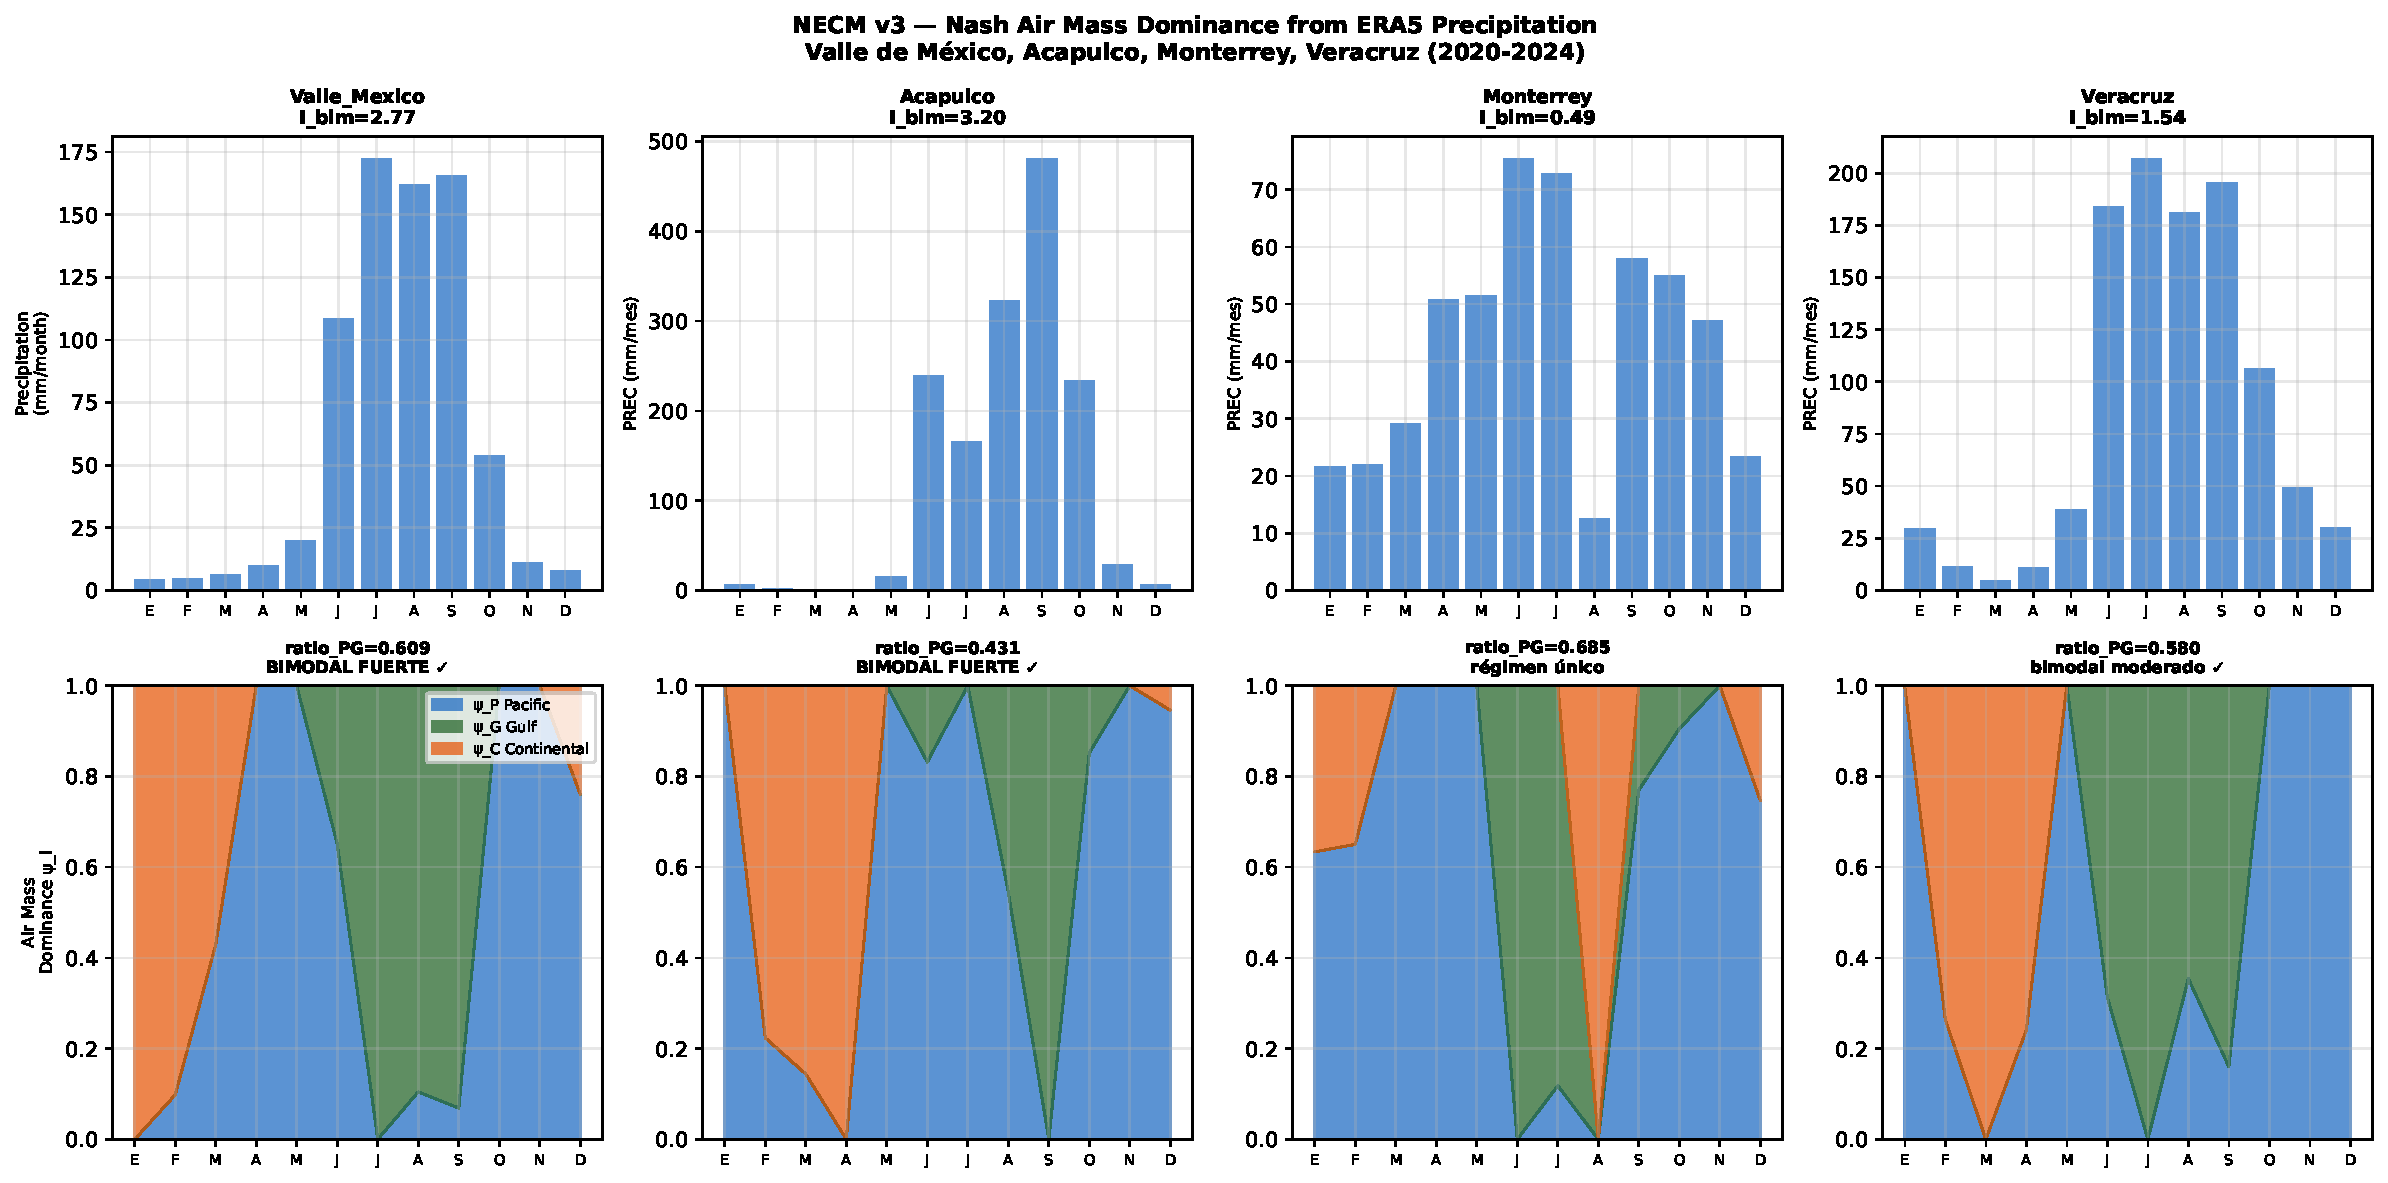
\includegraphics[width=\textwidth]{Fig5_NECM_v3_multiregion.pdf}
\caption{NECM proof of concept for four Mexican regions (ERA5, 2020--2024).
\textit{Top row}: monthly precipitation cycle (mm/month).
\textit{Bottom row}: Nash air mass dominance fractions $\psi_P$ (Pacific,
blue), $\psi_G$ (Gulf, green), and $\psi_C$ (Continental, orange).
Monterrey is correctly classified as unimodal; all other regions show
bimodal structure consistent with known climatology.}
\label{fig:multiregion}
\end{figure}

\section{Research Agenda}

The Super-Gap identified in Section~3 and the NECM framework proposed
in Section~4 together support a coherent research agenda of seven
articles, each addressing a distinct sub-gap confirmed by the Scopus
analysis:

\textbf{Art.C0} (this paper): CrossDomain gap analysis. Establishes
the literature void and proposes the NECM framework.
Target: \textit{Geoscientific Model Development} (Q1, IF~6.9).

\textbf{Art.C1}: Nash equilibrium for competing atmospheric air masses
— theoretical derivation from thermodynamic first principles.
Gap: S07~=~0, S17~=~0.
Target: \textit{Journal of the Atmospheric Sciences} (Q1).

\textbf{Art.C2}: Regional Fokker-Planck climate equation with
topographic prior — extension of Debussche~(2012) to regional scales
with Mexican orography.
Gap: S10~=~0, S16~=~0.
Target: \textit{Climate Dynamics} (Q1).

\textbf{Art.C3}: LeanFour2021 formal verification of NECM Propositions 1--3.
Gap: S11~=~0, S18~=~0, S24~=~0.
Target: \textit{Formal Aspects of Computing} (Q1).

\textbf{Art.C4}: Conceptual bridge from Nash-diplomatic to Nash-physical
climate models — a critical review of the disciplinary barrier.
Gap: S07~=~0 combined with S03~=~70.
Target: \textit{WIREs Climate Change} (Q1, review journal).

\textbf{Art.C5}: Physics-informed neural networks as residual correctors
of the Nash-EDE model — subordinating ML to theory.
Gap: S05~=~62 papers exist but none use Nash as physical backbone.
Target: \textit{npj Climate and Atmospheric Science} (Q1).

\textbf{Art.C6}: Empirical validation of NECM using SMN station
network and ERA5 reanalysis~\citep{Hersbach2020} over Mexico, 1980--2025.
Gap: S01~=~48 papers exist but none use Nash or EDE framework.
Target: \textit{International Journal of Climatology} (Q1).


\section{Discussion}

\subsection{Why Nash Never Reached Atmospheric Physics}

The thematic analysis of Section~3.5 reveals a consistent disciplinary
barrier: Nash equilibrium entered climate science through economics and
political science — domains where human strategic behavior is central —
and never crossed into atmospheric physics, where the ``players'' would
be physical entities (air masses, pressure systems) rather than agents
with preferences. This barrier is not mathematical but sociological:
the game-theory community and the atmospheric dynamics community read
different journals, attend different conferences, and share no common
vocabulary for formalizing air mass competition.

The opportunity cost of this barrier is significant. \citet{Debussche2012}
established that the 3D stochastic primitive equations are
well-posed — a result directly usable as the mathematical backbone of
NECM — yet this paper has 65 citations, none from the game-theory
community. Majda~(2005) derived a Fokker-Planck equation for planetary
waves — again directly relevant — with 49 citations, none connecting
to Nash equilibrium. The mathematical pieces existed in parallel for
over a decade without convergence.

\subsection{SCIFLOW as a Replicable Gap-Discovery Methodology}

The CrossDomain-Matrix methodology used here is a general tool for
identifying unexplored mathematical intersections in any scientific
domain. The key design principle is the four-level query structure:
confirming base-field activity at Level~1 ensures that identified gaps
are bounded by active literature, not by absence of interest. The false
positive detection protocol (Section~2.4) is essential for queries
involving polysemous terms such as ``Nash'' (equilibrium vs.
Nash-Sutcliffe index) and ``Lean'' (theorem prover vs. lean season).

\subsection{Limitations}

Four limitations of this analysis should be noted. First, the corpus
is restricted to Scopus-indexed literature; relevant work in conference
proceedings, technical reports, or non-indexed journals may be absent.
Second, the thematic classification is keyword-based and may
misclassify papers with non-standard terminology. Third, the NECM
framework proposed in Section~4 is theoretical; its empirical validity
depends on Art.C6 validation. Fourth, the coupling parameters
$\gamma_{ij}$ and seasonal temperatures $T_{m,i}$ must be estimated
from data; their identifiability from available observations is not
yet established.


\section{Conclusions}

We have presented a systematic cross-domain gap analysis of 187
peer-reviewed articles spanning six knowledge domains relevant to
regional climate prediction. Using the SCIFLOW CrossDomain-Matrix
methodology with 24 structured Scopus queries in four specificity
levels, we find:

\begin{enumerate}
\item Eleven confirmed literature gaps, including four at the
      highest specificity level (Super-Gap).
\item Nash equilibrium appears in 70 climate papers but exclusively
      in diplomatic and economic contexts; it has never been applied
      as a physical principle governing atmospheric air mass dynamics.
\item Stochastic primitive equations for the atmosphere exist
      mathematically~\citep{Debussche2012,Majda2006} but without
      Nash game-theoretic structure or formal verification.
\item Formal verification has never been applied to any climate model.
\item The triple intersection of Nash equilibrium, stochastic field
      theory, and formal verification applied to regional climate
      prediction contains zero papers in the Scopus database as of
      June 2026.
\end{enumerate}

We propose the Nash-EDE Climate Model (NECM) as the theoretical
framework that fills this intersection, and outline a research agenda
of seven articles. The central falsifiable prediction — that the
ratio $\gamma_{PG}/\sqrt{\beta_P\beta_G} \in [1.2, 2.5]$ distinguishes
regions with stable bimodal precipitation from aperiodic regimes —
is testable with existing ERA5 and SMN data.

The disciplinary barrier between game theory and atmospheric physics
has persisted for decades despite the mathematical pieces being
available. SCIFLOW's CrossDomain-Matrix methodology is designed
precisely to make such barriers visible and crossable.

\bibliographystyle{plainnat}
\bibliography{Art_C0_referencias}
\end{document}
